\section*{Introduction}

\textbf{Motivation:} Single-cell RNA-seq is a promising technique that profiles transcriptomes over a plethora of cell types. By measuring individual cells, rather than averaged tissue types, scRNA-seq can uncover biological mechanisms that is not observed by the average behaviors of a bulk of cells  \citep{wang2017vasc}. However, despite improvements in measuring technologies, factors including amplification bias, cell cycle effects \citep{buettner2015computational}, etc. lead to substantial noise in scRNA-seq experiments. The low RNA capture rate leads to failure of detection of an expressed gene resulting in a ``false" zero count observation, defined as dropout event; which potentially corrupts the underlying biological signal \cite{eraslan2018single}. One such scRNA-seq data set is from the 10x genomics project that profiles 1.3 M embroynic brain cells of two mice. It represents cells from cortex, hippocampus and subventricular zone of two mice at 18 days post conception which is an invaluable resource to study gene dynamics during an important development stage. However, the corruption induced by dropout events compromises our ability to use analytical techniques to extract meaningful patterns. 

We utilize a 20 K sampled version (21 K genes $\times$ 20 K single cells) of the 1.3 M embroynic brain cells data-set and use a simple decision tree algorithm to establish a baseline performance when minimal data-transformation were applied. For denoising /imputation, current approaches (like MAGIC) rely on using the correlation structure of single-cell gene expression data, leveraging similarities between cells and/or genes that does not scale well; or has explicit / implicit linearity assumption that may miss complex non-linear patterns \citep{eraslan2018single}. Deep-learning auto-encoders can learn the underlying complex manifold, that represents the biological processes and/or cellular states and utilize that to reduce the high dimensional data space to significantly lower dimensions \citep{moon2017manifold}. However, using an auto-encoder as is may fail due to the noise model not being adapted to typical scRNA-seq noise. One such autoencoder DCA -- deep count autoencoder facilitates non-linear embedding of cells and uses scRNA-seq data specific loss function based on negative binomial count distributions which offers adaptive learning and encoding of the data manifold \citep{eraslan2018single}. To illustrate the difference, we utilize DCA and MAGIC to denoise / impute the dataset and then re-apply the classical decision tree algorithm to learn if gene expression dynamics can infer different cell regions.

\section*{Problem definition}
We solve the following four problems in this report. 1) Normalize and filter the single cell data by removing genes with low coefficient of variation and poor quality cells -- baseline, 2) cluster 20 K single cells into three groups representing different spatial location on the mouse brain to get class labels, 3) apply DCA and MAGIC transformations on the normalized data-set and 4) use Decision Tree classifier to classify cell-regions based on gene expression for the baseline and the two transformed datasets.

\section*{Solution}

\subsection*{Data source}
We are using a 20 K single cell subset of the Cell Ranger 1.3.0 dataset from the 10x Genomics project that provides 1.3 M Brain Cells from E18 Mice which consists of cells from cortex, hippocampus and subventricular zone of two E18 mice. The data was retrieved from \href{https://support.10xgenomics.com/single-cell-gene-expression/datasets/1.3.0/1M_neurons}{\textcolor{blue}{support.10xgenomics.com}}. Prior any transformation, the data has about 21 K genes which we would use as features and 20 K single cells which we would utilize as observations.

\begin{figure*}
\begin{framed}
\begin{minipage}{\linewidth}
\begin{minipage}[t]{0.48\linewidth}
\vspace{0pt}
\textsf{a)}\\
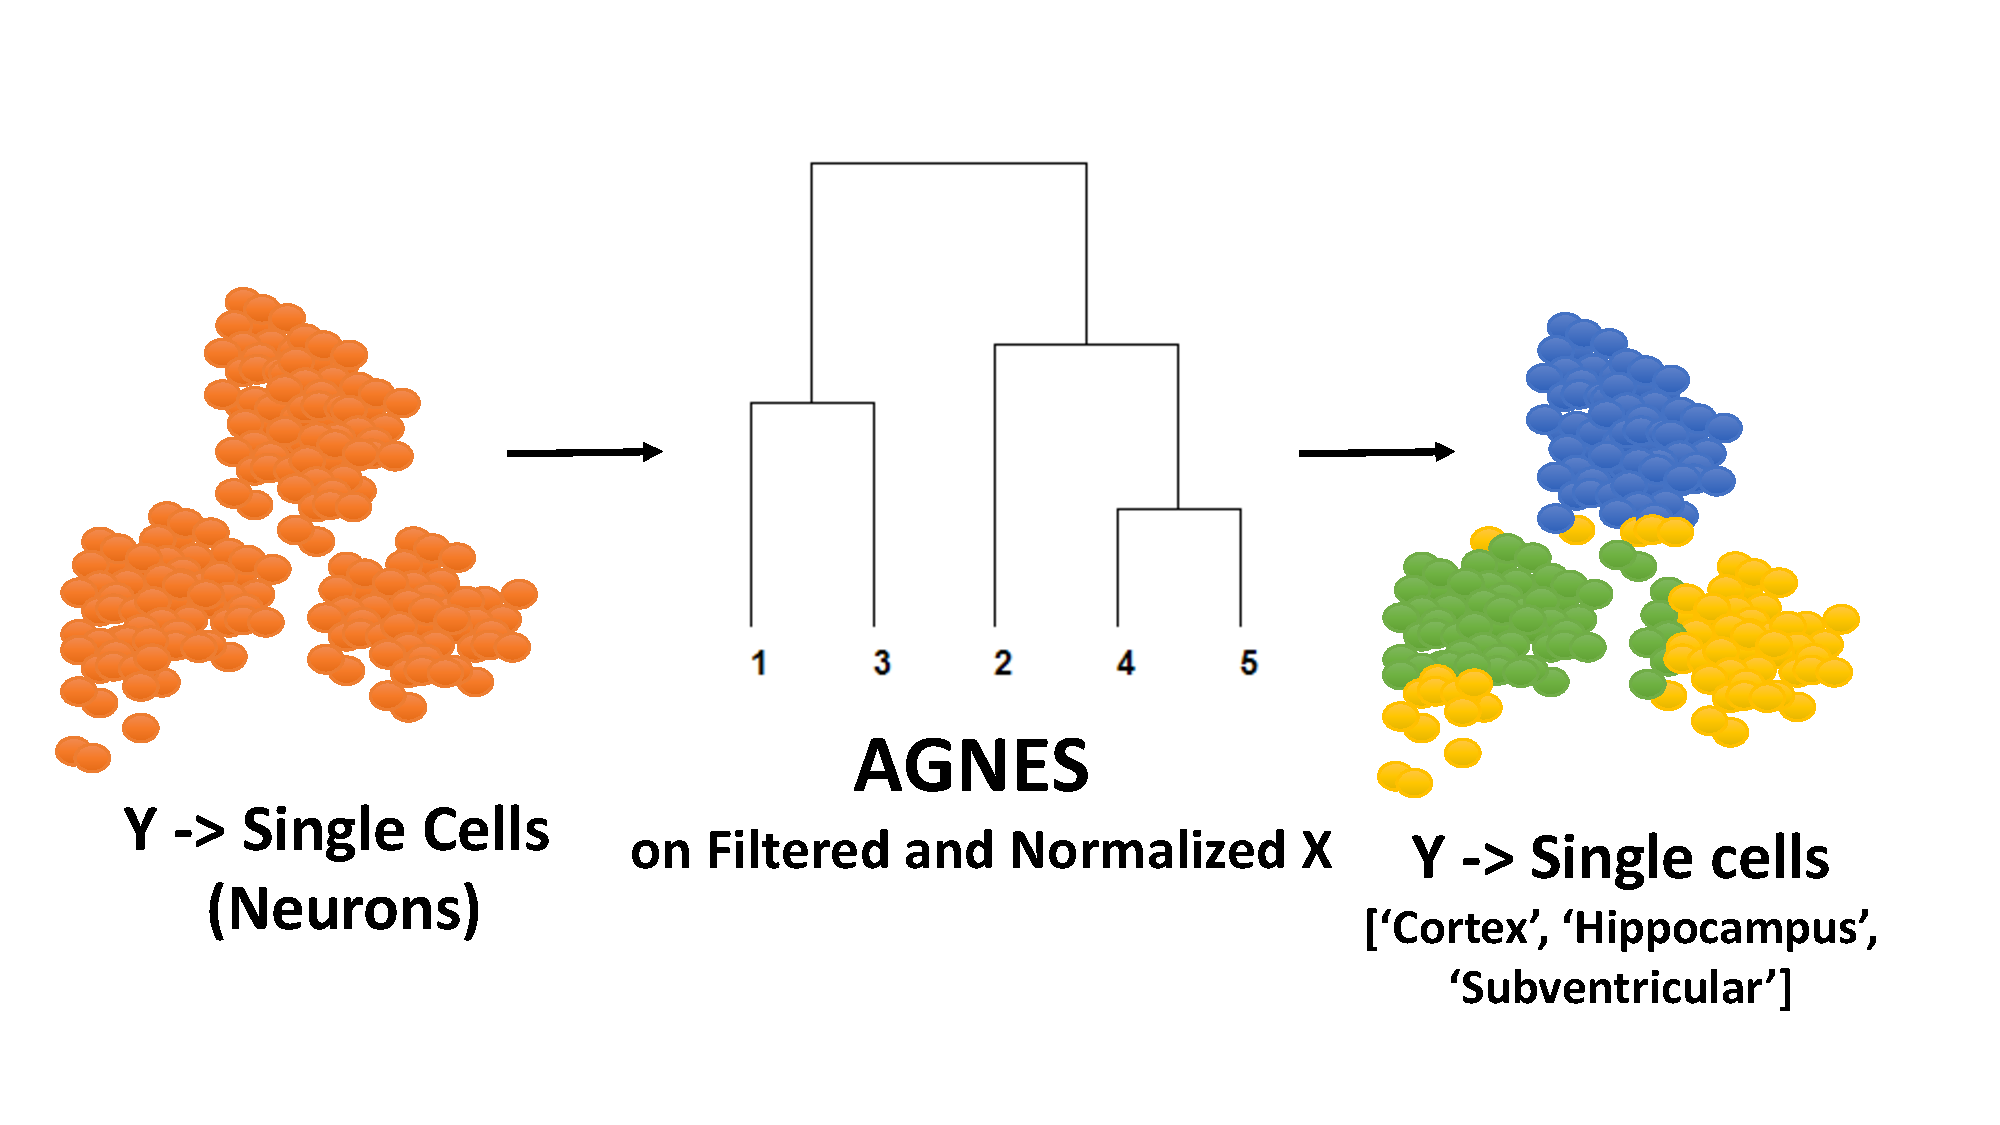
\includegraphics[width=\linewidth]{agnes.pdf}
\end{minipage}
\begin{minipage}[t]{0.48\linewidth}
\vspace{0pt}
\textsf{b)}\\
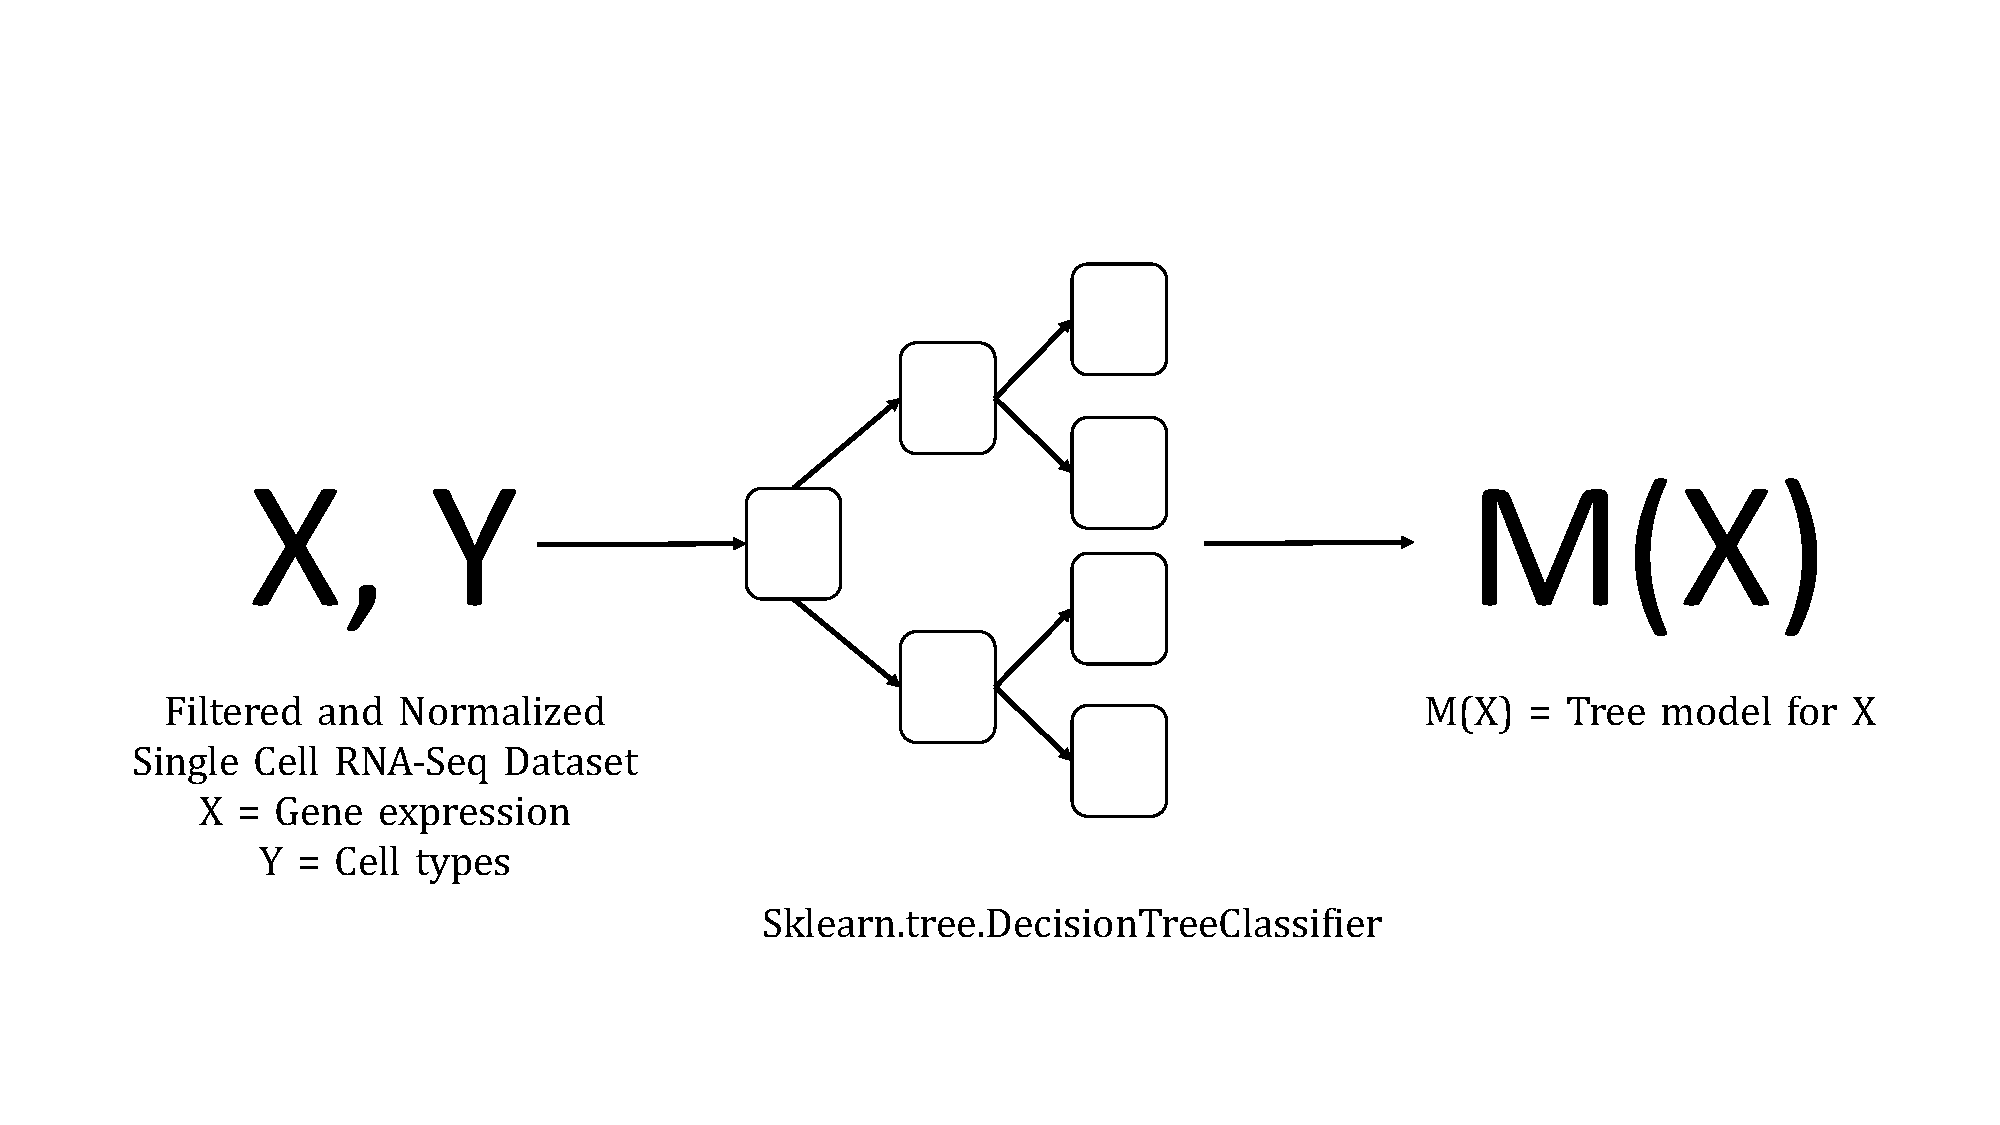
\includegraphics[width=\linewidth]{without_autoencoding.pdf}
\end{minipage}
\end{minipage}
\begin{minipage}{\linewidth}
\begin{minipage}[t]{0.48\linewidth}
\vspace{0pt}
\textsf{c)}\\
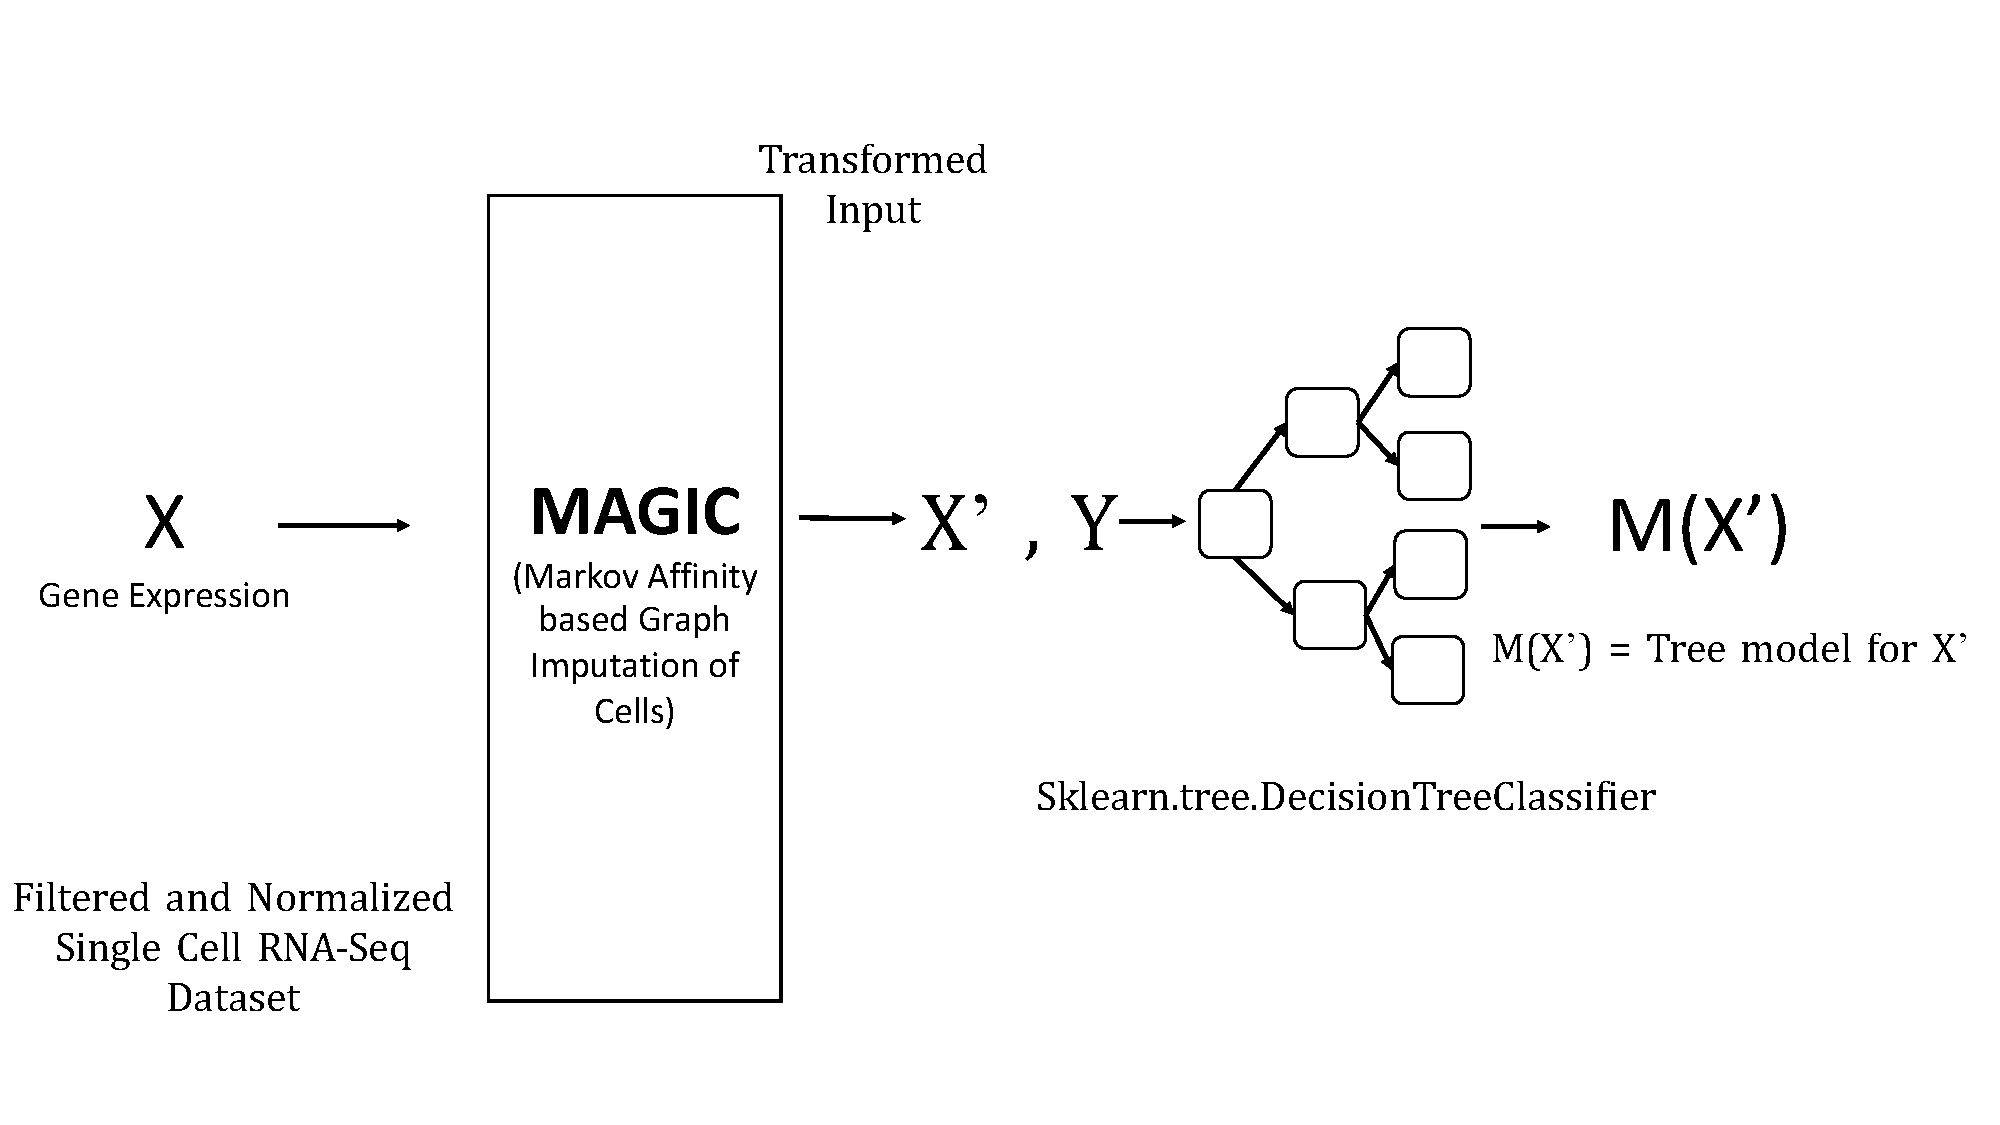
\includegraphics[width=\linewidth]{with_magic.pdf}
\end{minipage}
\begin{minipage}[t]{0.48\linewidth}
\vspace{0pt}
\textsf{d)}\\
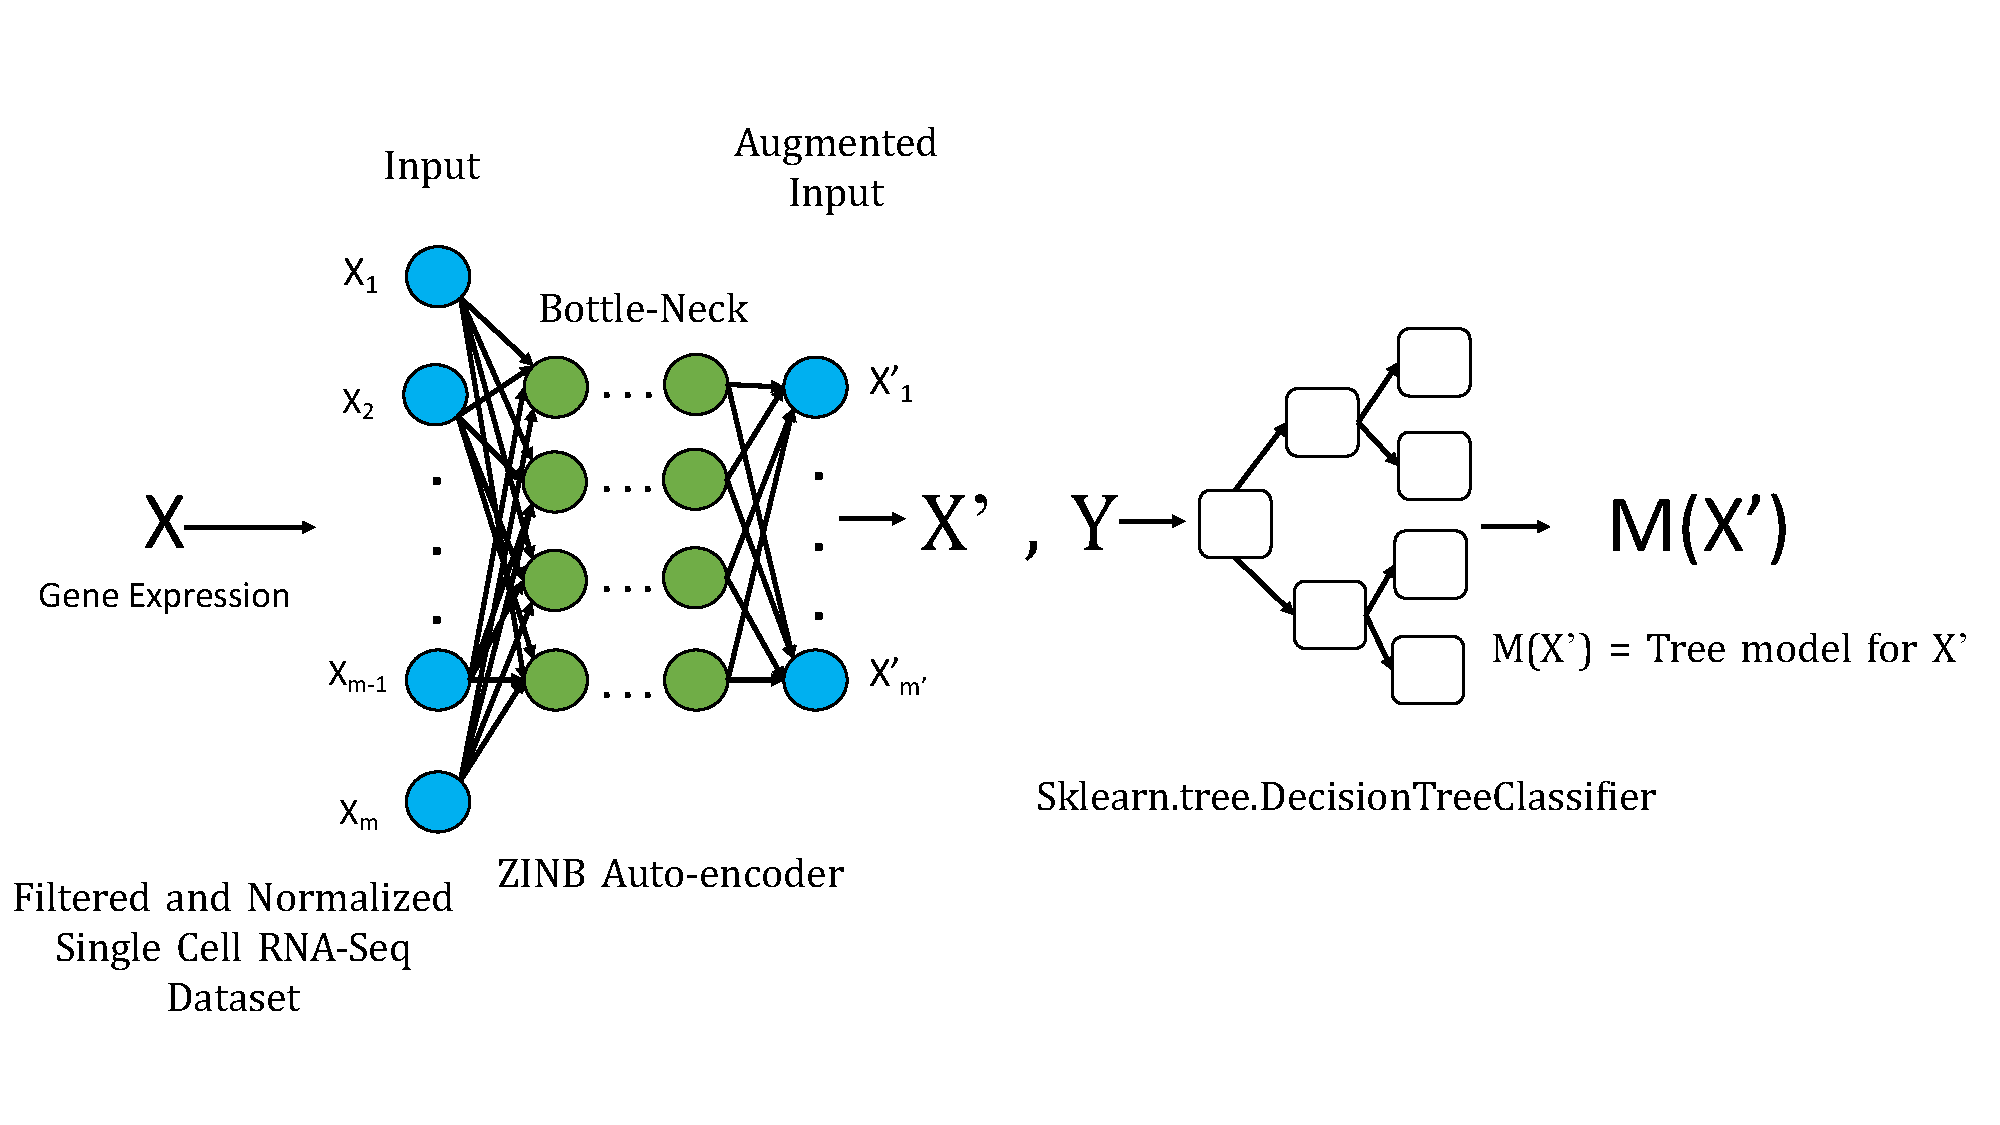
\includegraphics[width=\linewidth]{with_autoencoding.pdf}
\end{minipage}
\end{minipage}
\caption{a) After the data has been filtered and normalized, we use AGNES to cluster the cells based on feature (genes) similarity. b) After we have class labels / cell clusters, the filtered and normalized single cell data will be supplied as is to a sklearn decision tree algorithm. c) The filtered and normalized single cell data will be denoised / imputed using the ZINB DCA autoencoder and then the learned manifold X$^{'}$ will be supplied to the sklearn decision tree algorithm. d) The filtered and normalized single cell data will be denoised / imputed using MAGIC ( X$^{'}$ ) which will then be supplied to the sklearn decision tree algorithm.}
\end{framed}
\label{fig1}
\end{figure*}

\subsection*{Data filtration and normalization}

We closely followed the step by step workflow for low-level analysis of single-cell RNA-seq data \citep{lun2016step} for preliminary data cleaning and normalization. 

\subsubsection*{Filtration} 

Depending on the experimental setup, many genes would show little to no dynamics across collected cell types and thus it is beneficial to only focus on active genes. To measure gene activity, we computed the dispersion of each gene expression across all 20 K cell types by measuring their coefficient of variation $COV_g$ given by :

\begin{equation}
COV_g = \frac{\sigma_g}{\mu_g}
\end{equation}

where $\sigma_g$ represents the standard deviation of gene $g$ and $\mu_g$ represents the mean expression of gene $g$. A good threshold for a 'high' coefficient of variation, was computed as :

\begin{equation}
COV_g \geq \forall g \in G, M (COV_g) - 3 \cdot k \cdot | COV_g - M (COV_g) |
\end{equation}

that is, if the coefficient of variation $COV_g$ for a gene $g \in G$ ($G$ being the set of all 21 K genes) was considered good if it was higher than three median absolute deviation (MAD) ($k \cdot | COV_g - M (COV_g) |$) from the median $M (COV_g)$. Where $k$ is a scale factor given by $1 / \phi_g$ ($\phi_g$ being the upper quartile of the gene expression distribution).

\begin{figure}
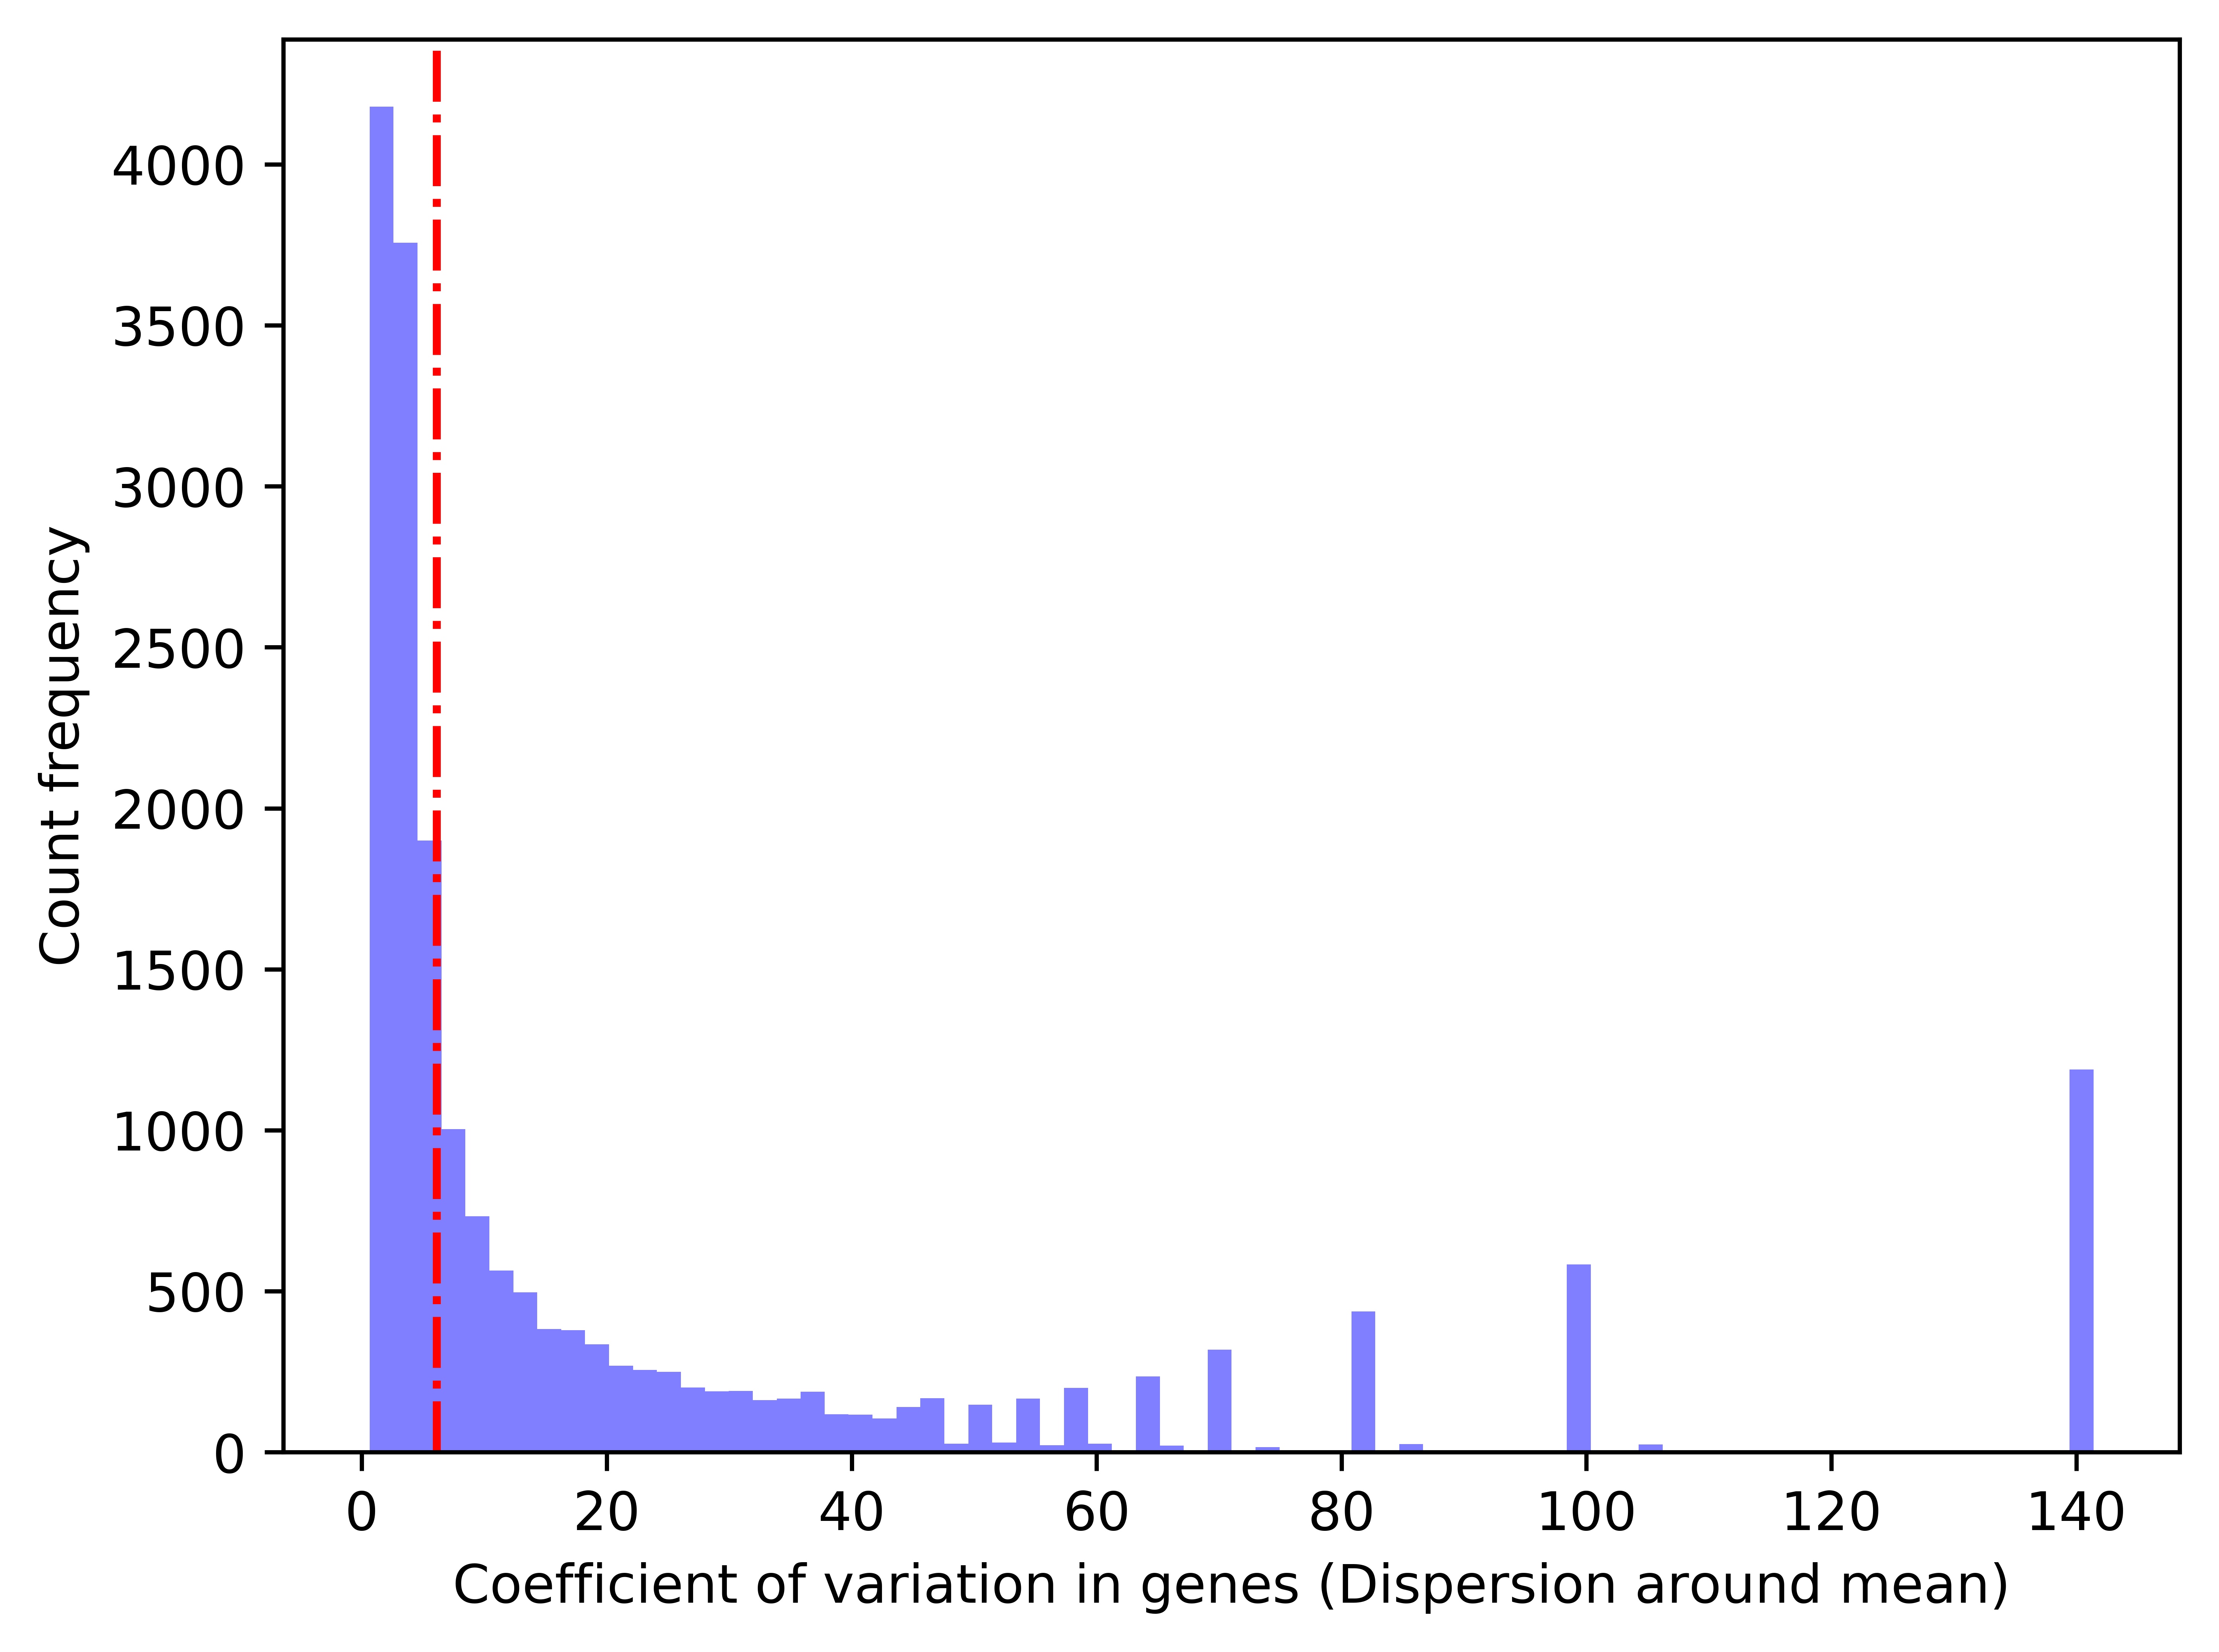
\includegraphics[width=\linewidth]{sc_20k_mouse_neurons_coef_of_variation_cutoff.png}
\caption{Coefficient of variation distribution for all genes}
\end{figure}

Figure~2 shows the distribution of coefficient of variation ($COV_g$) for all $g \in G$. The red dotted line shows the chosen cutoff. All genes with a coefficient of variation higher than the chosen cutoff were kept, while others were removed.

Since the Single Cell technology is massively high throughput, it is easier to capture poor quality / broken cells. We want to remove these cells from consideration. The most basic method to detect poor / broken cell is to compute the log feature count for each cell -- which is the log of the number of non-zero gene expressed in that cell (we denote it by $LFC_c$). Again to choose a good threshold for 'high' feature count we computed the following :

\begin{equation}
LFC_c \geq \forall c \in C, M ( LFC_c ) - 3 \cdot k \cdot | LFC_c - M ( LFC_c ) |
\end{equation}

that is, if the log feature count $LFC_c$ for a cell $c \in C$ ($C$ being the set of all 20 K cells) was considered good if it was higher than three median absolute deviation (MAD) ($k \cdot | LFC_c - M ( LFC_c ) |$) from the median $M ( LFC_c )$. Where $k$ is a scale factor given by $1 / \phi_c$ ($\phi_c$ being the upper quartile of the cell expression distribution).

\begin{figure}
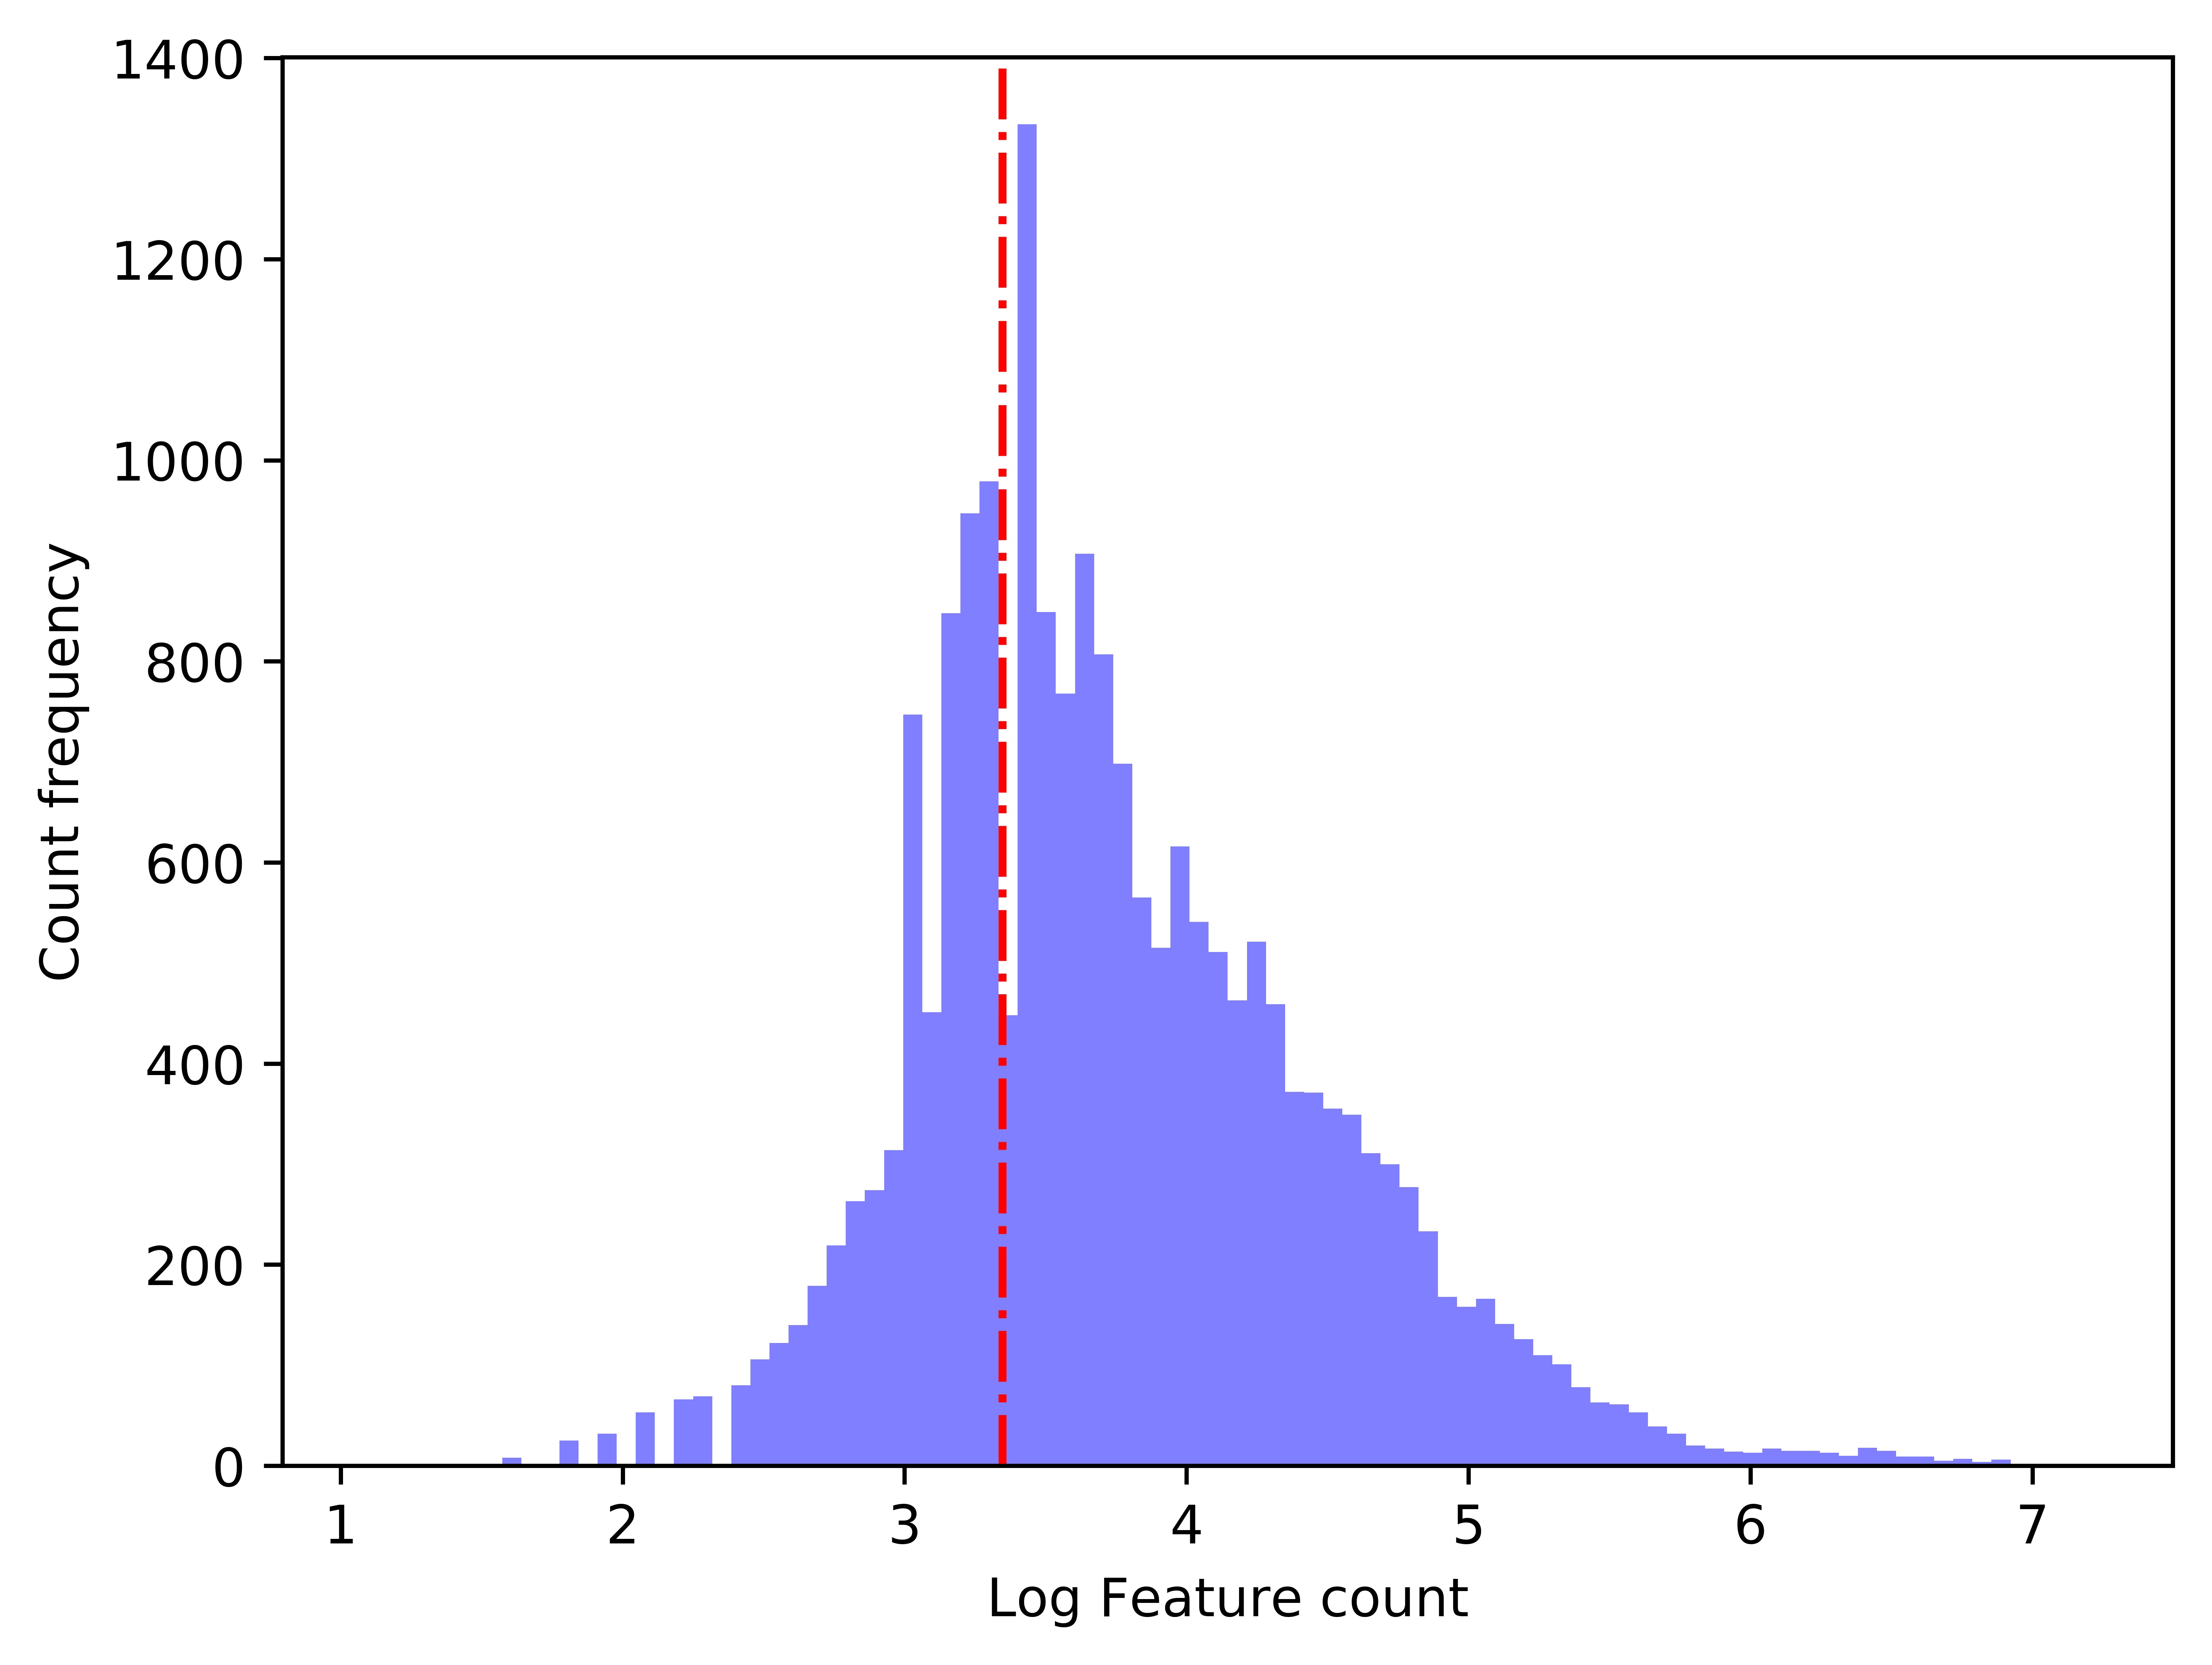
\includegraphics[width=\linewidth]{sc_20k_mouse_neurons_sample_feature_count_cutoff.png}
\caption{Log feature count distribution for all cells}
\end{figure}

Figure~3 shows the distribution of log feature count ($LFC_c$) for all $c \in C$. The red dotted line shows the chosen cutoff. All cells with a log feature count higher than the chosen cutoff were kept, while others were removed. Post filtration, we were left with about 10 K genes and 14 K single cells.

\subsubsection*{Normalization}

Normalization becomes necessary as the Single Cell RNA - Seq data is blind to the stage of the cell it captures. Some cells could be nascent whereas others could be matured. Normalization by feature count was recently employed in a single cell analysis \citep{carter2018single} of developing mouse cerebellum. Thus, we used a similar normalization technique for our data, given by :

\begin{equation}
X[c, g] = \forall c, g \in C, G; log ( X [c, g] * \left[ M (X [ c, . ] ) /  X [c, .] \right] )
\end{equation}

where $X [c, g] $ represents gene $g \in G$ and cell $c \in C$ in $X$, $X [c, .]$ represents the row sum of cell $c$ (sum of all gene expression measured in cell $c$) and $M (X [ c, . ] )$ represents the median of all $X [c, .], c \in C$.

\subsection*{Hierarchical clustering of single cells}

The data-set we decided to utilize, did not capture any meta information on cell types / regions and thus to be able to do classification, we required class labels. The single cell data of developing mouse cerebellum \citep{carter2018single} generated by St. Jude Children Hospital had a similar experimental design, where meta cell information was missing. They utilized prior knowledge and hierarchical clustering to cluster the single cells into various cell types.

Following a similar approach,  we clustered the single cells using the AGNES implementation of hierarchical clustering offered by \texttt{scipy} library in python. The choice of metric to compute the pairwise distance was `euclidean' and `ward' for computing the distance between the newly formed clusters. `fcluster' using 'maxclust' was used to cut the dendogram into three clusters.

\begin{figure}
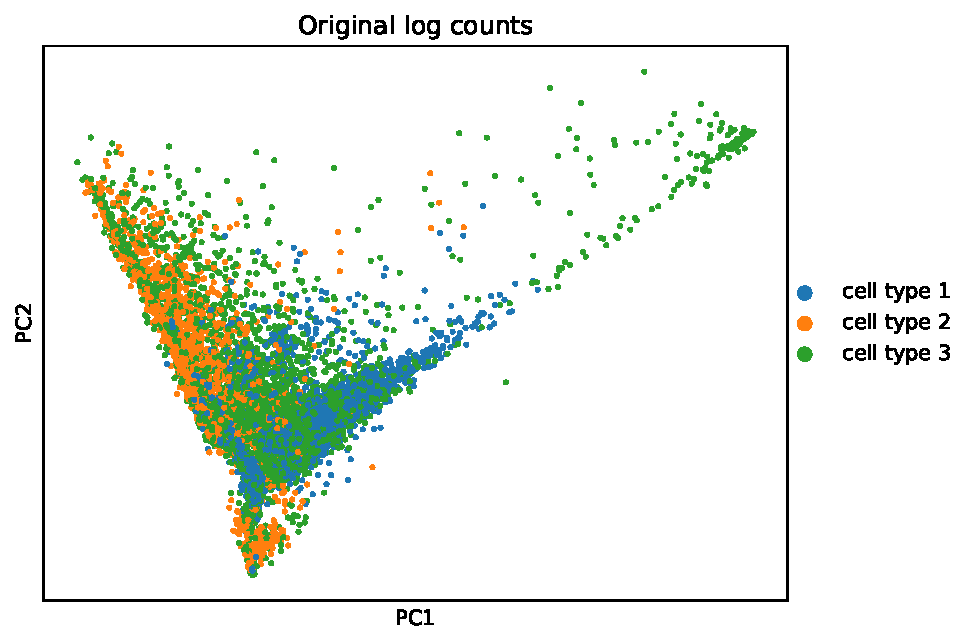
\includegraphics[width=\linewidth]{pca_og_log_counts.pdf}
\caption{PCA of the filtered and normalized dataset}
\end{figure}

Figure~4 shows the first two principal components (linear combination of genes) of the filtered and normalized data. The three colors represent the clustered cell types / regions. It can be seen that the data is not a spherical blob with no separability and does show potential to be classified into different cell types / regions.

\subsection*{Classification using Decision Tree Classifier}

For classification, we used the decision tree implementation offered by `sklearn' python library. All parameters were set at their default values, except two regularization parameters, \texttt{min\_samples\_leaf} and \texttt{min\_samples\_split} that were set at 100 and 1000 respectively. The reason for choosing high numbers here was because the data has many observations and thus, allowing small split and leaf size may end up over-fitting the data.

\subsection*{ZINB DCA Autoencoder transformation}

One of the advanced pre-processing strategy we used was the zero-inflated negative binomial (ZINB) DCA auto-encoder \citep{eraslan2018single} that claims to denoise the single cell data by learning the manifold of the data. Precisely, the authors of the DCA auto-encoder assume that each gene in the single cell data can be expressed as (or follows) zero-inflated negative binomial distribution. While it may be a bold assumption, we believe it is reasonable as the dropout event induces such behavior onto the single cell data. 

The DCA deep auto-encoder uses CNN from the tensor flow package in python and learns the ZINB parameters $\mu$ (mean), $\theta$ (dispersion) and $\phi$ (point mass) \citep{eraslan2018single} for each gene. After the parameters are learned, each gene is then transformed / imputed using the ZINB distribution.

The DCA API in python was used to transform the data. When applying this method, we closely followed the tutorial provided by the authors on their github page.

\begin{figure}
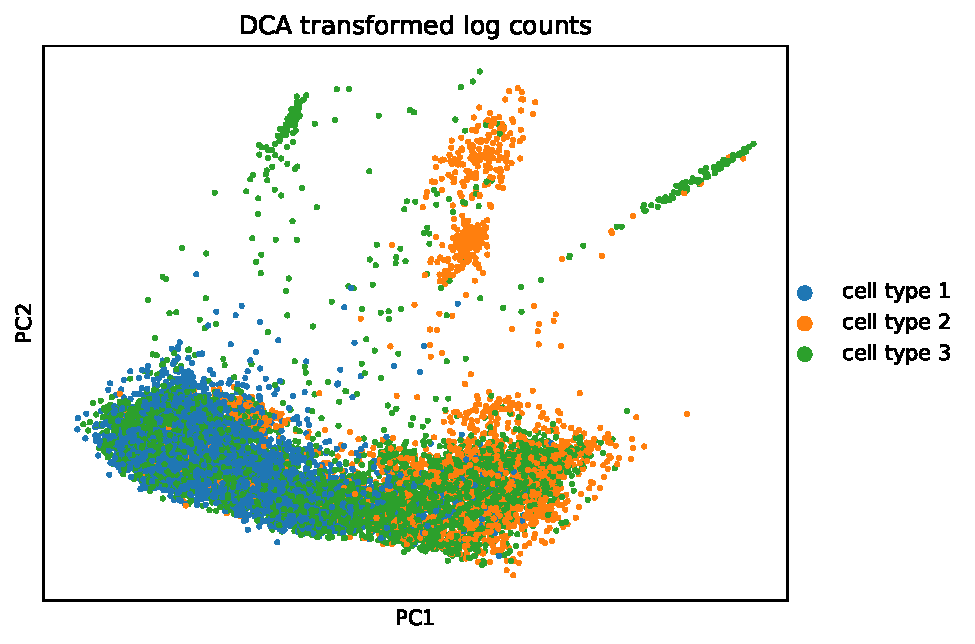
\includegraphics[width=\linewidth]{pca_dca_log_counts.pdf}
\caption{PCA of the DCA transformed dataset}
\end{figure}

Figure~5 shows the first two principal components (linear combination of genes) of the DCA transformed data. The three colors represent the clustered cell types / regions. It can be seen that this transformation offers more separability compared to the baseline.

\subsection*{MAGIC transformation}

Markov Affinity based Graph Imputation of Cells \citep{van2018recovering} is a relatively known denoising / imputation method that relies on cell correlation to share information among similar cells, captured by correlation and k-nearest neighbors algorithm, and uses this information to denoise / impute cell data.

The MAGIC class in python was used to transform the data. When applying this method, we closely followed the tutorial provided by the authors on their github page.

\begin{figure}
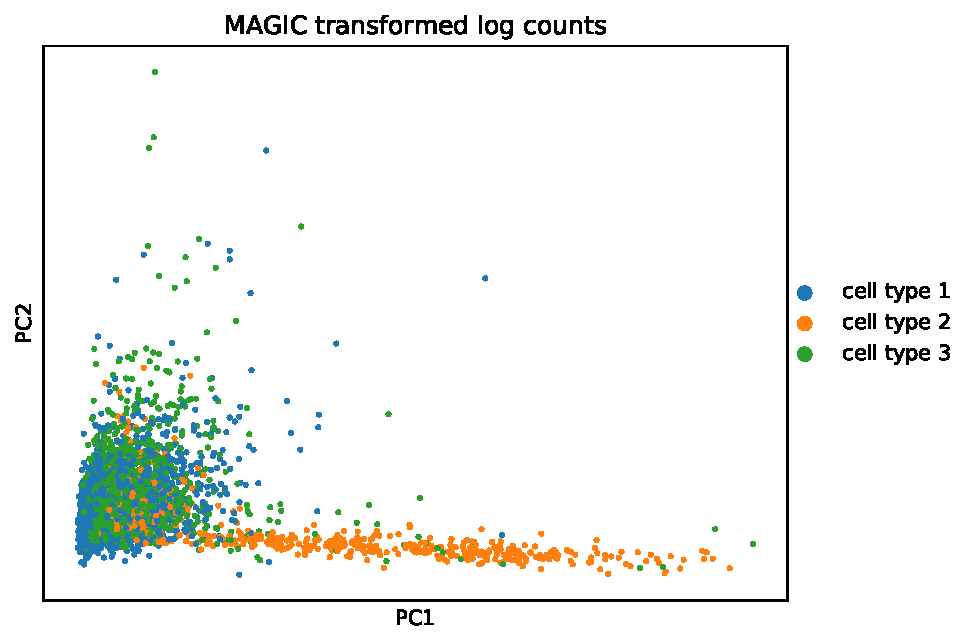
\includegraphics[width=\linewidth]{pca_magic_log_counts.pdf}
\caption{PCA of the MAGIC transformed dataset}
\end{figure}

Figure~6 shows the first two principal components (linear combination of genes) of the MAGIC transformed data. The three colors represent the clustered cell types / regions. It can be seen that this transformation offers less separability between cell type 1 and cell type 3.

\section*{Results}

Here we present decision tree 10-fold CV accuracies for three separate representation of the single-cell dataset. 1) Filtered and normalized data -- baseline, 2) DCA transformed data and 3) MAGIC transformed data. The data was standardized using `StandardScalar' method in `sklearn'.

\begin{table}[!hbtp]
\begin{tabular}{|l|c|c|c|c|c|c|c|c|c|c|}
\hline
\textbf{D} & \textbf{1} & \textbf{2} & \textbf{3} & \textbf{4} & \textbf{5} & \textbf{6} & \textbf{7} & \textbf{8} & \textbf{9} & \textbf{10} \\\hline
1 & 0.81 & 0.81 & 0.78 & 0.83 & 0.82 & 0.81 & 0.84 & 0.82 & 0.84 & 0.82 \\
2 & \textbf{0.87} & \textbf{0.85} & \textbf{0.88} & \textbf{0.85} & \textbf{0.86} & \textbf{0.86} & \textbf{0.86} & \textbf{0.85} & \textbf{0.85} & \textbf{0.88} \\
3 & 0.82 & 0.80 & 0.78 & 0.81 & 0.81 & 0.80 & 0.78 & 0.80 & 0.78 & 0.78 \\\hline
\end{tabular}
\caption{Accuracy of three data-representation over 10-fold cross validation.}
\end{table}

The performance of decision tree on DCA transformed data is consistently the best shows significant improvement over the baseline in many cases. MAGIC on the other hand performs consistently worse than the baseline with few exceptions.

\section*{Discussion}

Empirical evidence suggests that the underlying assumption of DCA, genes following ZINB distribution, better captures the dynamics in the data. Interestingly, the baseline itself is not too bad, given the fact that the cell-types being classified here may not be the true class labels. The relatively worse performance of MAGIC can be explained. MAGIC relies on correlation and KNN measures to find out similar cells, this can be very subjective to non-uniform feature expression distribution within a cell. Also, two truly identical cell types can be far apart from each other coming from different stages and/or age, as well as two completely dissimilar cells could be quite close but may represent completely different cellular functionality. which should not be used to infer missing or misinterpreted expression values. Given huge sample size (probably 1.3 M neurons) the likelihood of finding the true neighbor (highly similar cell) would be high, however, it does not seem to work for 20 K single cells.